\section{TSP}

Badania dla problmu TSP zostały wykonane z użyciem instancji problemu \textit{kroa100}, o rozwiązaniu 21282. 


\begin{figure}[H]
	\centering
	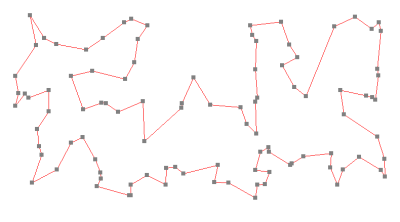
\includegraphics[scale=0.6]{tsp/kroA100_optimal}
	\caption{Rozwiązanie optymalne problemu kroa100}
\end{figure}

\paragraph{Parametry}
Badania wpływu parametrów na uzyskiwane wyniki zostały przeprowadzone dla parametrów określających szansę na krzyżowanie oraz wielkość populacji. Wyniki zostały uśrednione z 15 przebiegów algorytmu. Ustawienia: 

\begin{itemize}
	\item popSize = 50
	\item maxIter = 500
	\item run = 100
\end{itemize}

Pozostałe parametry posiadały wartość domyślną.

\subsection{Wyniki}

\begin{figure}[H]
	\centering
	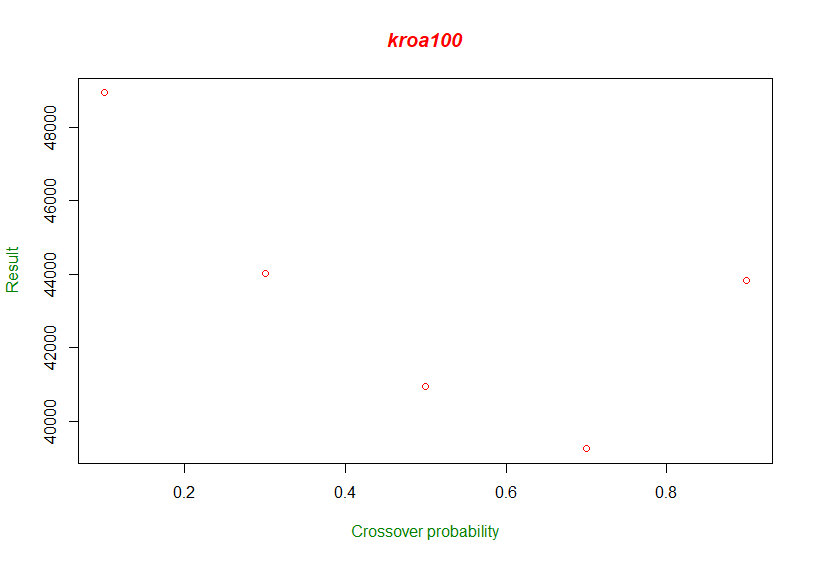
\includegraphics[scale=0.6]{tsp/kroa100_pcross}
	\caption{Rezultat optymalizacji dla różnych wartościach prawdopodobieństwa krzyżowania}
\end{figure}

\begin{figure}[H]
	\centering
	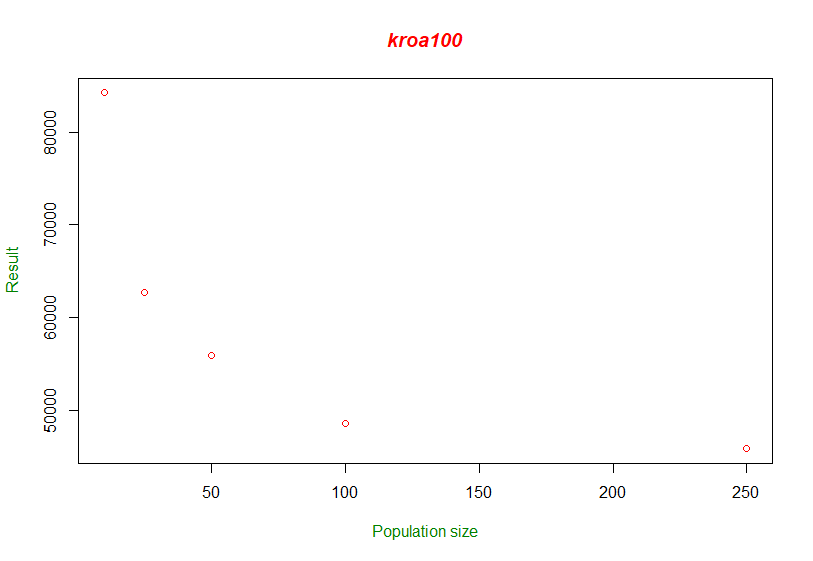
\includegraphics[scale=0.6]{tsp/kroa100_popSize}
	\caption{Rezultat optymalizacji dla różnych wielkości populacji}
\end{figure}

\begin{figure}[H]
	\centering
	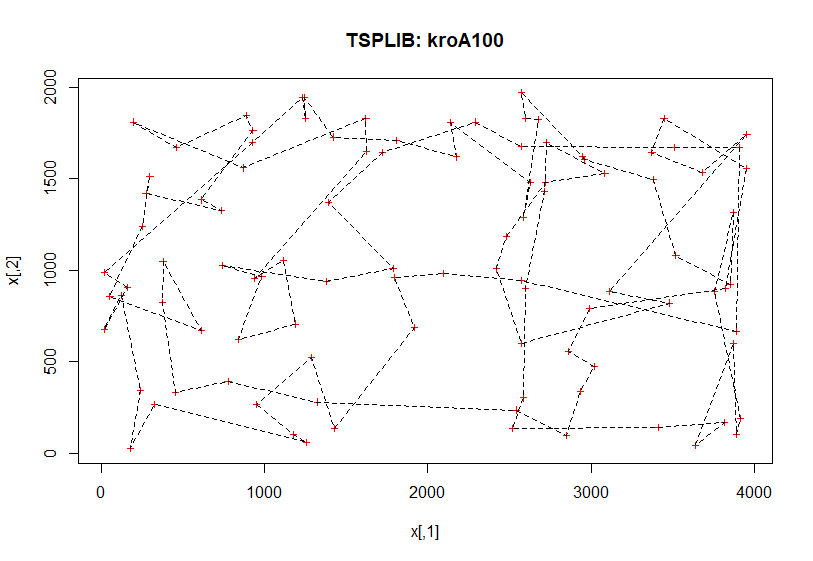
\includegraphics[scale=0.6]{tsp/40k}
	\caption{Przykładowa trasa o długości 40 000}
\end{figure}

\subsection{Wnioski}
Zwiększenie parametru \textit{pcrossover} powyżej wartości domyślnej 0,8 powoduje spadek wyników osiąganych przez algorytm.

Wielkość populacji ma bezpośredni wpływ na osiągane rezultaty - jej zwiększanie poprawia końcowy wynik. Zwiększanie tego parametru powoduje jednak znaczące wydłużenie czasu działania algorytmu, natomiast zysk stopniowo się zmniejsza. W czasie przeprowadzania badań najkorzystniejszą wielkością populacji okazało się 100 - powyżej tej wartości długość obliczeń dla pojedynczej iteracji jest zbyt duża. Kompromisem jest  zmniejszanie populacji a zwiększanie dopuszczalnej liczby maksymalnej iteracji. \\
Aby określić najkorzystniejsze parametry należałoby przeprowadzić badania algorytmu dla tych parametrów, porównując osiągane wyniki po zadanym czasie, np. 1 minuty.
